%% -*- Lecture -*-

\documentclass[11pt,aspectratio=169]{beamer}

\usepackage{rcstalk}
\usepackage{bytefield}

\usetheme{rcstheme}

\subtitle{Lecture 7: Virtual memory HW}
\topic{Virtual memory HW}

\begin{document}

\maketitle

\begin{slide}{Want processes to co-exist}
\centerline{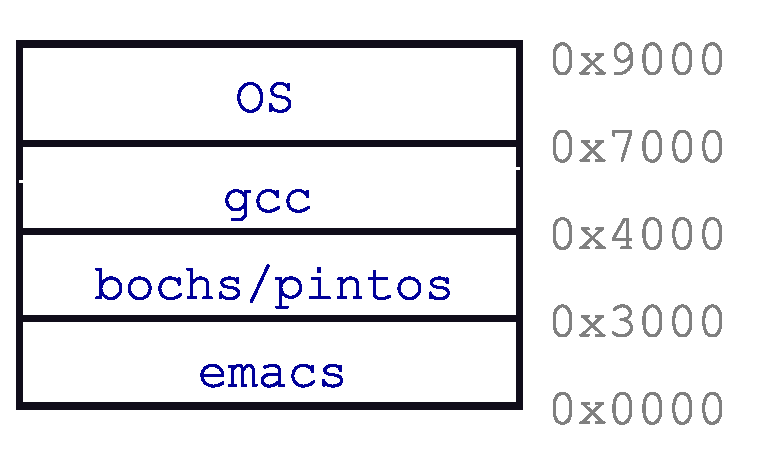
\includegraphics[height=1.5in]{figs/coexist}}

\medskip

\itms{
  \item Consider multiprogramming on physical memory
  \ittms{
\item What happens if emacs needs to expand?
\item If emacs needs more memory than is on the machine??
\item If emacs has an error and writes to address 0x7100?
\item When does gcc have to know it will run at 0x4000?
\item What if emacs isn't using its memory?
  }
}
\end{slide}

%% \begin{slide}{\large Multiprogramming on physical memory}
%% \itms{
%%   \item Makes it hard to allocate space contiguously
%%   \ittms{
%%     \item Convenient for stack, large data structures, etc.
%%   }
%%   \item Need fault isolation between processes
%%   \ittms{
%%     \item (Even Microsoft now seems to believe this\ldots)
%%   }
%%   \item Processes can consume more than available memory
%%   \ittms{
%%     \item Dormant processes (wating for event) still have core images
%%   }
%% }
%% \end{slide}

\begin{slide}{Issues in sharing physical memory}
\itms{
  \item \Red{Protection}
  \ittms{
    \item A bug in one process can corrupt memory in another
    \item Must somehow prevent process\ $A$ from trashing $B$'s memory
    \item Also prevent $A$ from even observing $B$'s memory
  (ssh-agent)
  }
  \item \Red{Transparency}
  \ittms{
    \item A process shouldn't require particular physical memory bits
    \item Yes processes often require large amounts of contiguous
      memory (for stack, large data structures, etc.)
  }
  \item \Red{Resource exhaustion}
  \ittms{
    \item Programmers typically assume machine has ``enough'' memory
    \item Sum of sizes of all processes often greater than physical
  memory
  }
}
\end{slide}

\begin{slide}{Virtual memory goals}
\vspace{-2em}
  \centerline{\includegraphics[width=112mm]{vmhilevel}}
\vspace{-2em}
\itms{
  \item Give each program its own ``virtual'' address space
  \ittms{
    \item At run time, Memory-Management Unit relocates each load,
      store to actual memory\ldots\ App doesn't see physical memory
  }
  \item Also enforce protection
  \ittms{
    \item Prevent one app from messing with another's memory
  }
  \item And allow programs to see more memory than exists
  \ittms{
    \item Somehow relocate some memory accesses to disk
  }
}
\end{slide}

\begin{slide}{Virtual memory advantages}
\vspace{-1em}
\itms{
  \item Can re-locate program while running
  \ittms{
    \item Run partially in memory, partially on disk
  }
  \item Most of a process's memory may be idle (80/20 rule).  
  \ittms{
%\item[]\hspace*{-.3in}\includegraphics[width=4in]{figs/vmadv}
  \item[]\vspace*{-4em}\includegraphics[width=4in]{vmadv}\vspace*{-1em}
  \item Write idle parts to disk until needed
  \item Let other processes use memory of idle part
  \item Like CPU virtualization: when process not using CPU, switch \\
    (Not using a memory region? switch it to another process)
}
  \item Challenge: VM = extra layer, could be slow
}
\end{slide}

\begin{slide}{Idea 1: load-time linking}
\centerline{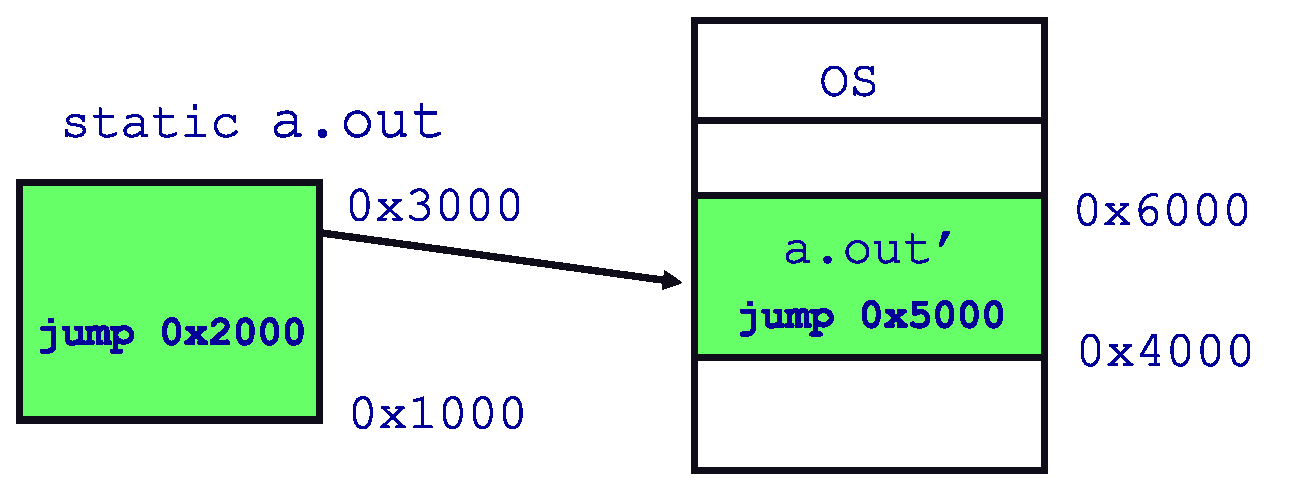
\includegraphics[height=1.3in]{figs/loadtime}}
\itms{
  \item \emph{Linker} patches addresses of symbols like
    \texttt{printf}
  \item Idea: link when process executed, not at compile time
  \ittms{
    \item Determine where process will reside in memory
    \item Adjust all references within program (using addition)
  }
  \item Problems?
\pause
  \ittms{
    \item How to enforce protection 
    \item How to move once already in memory (Consider: data pointers)
    \item What if no contiguous free region fits program?
  }
}
\end{slide}

\begin{slide}{Idea 2: base + bound register}
\vspace{-1em}
\centerline{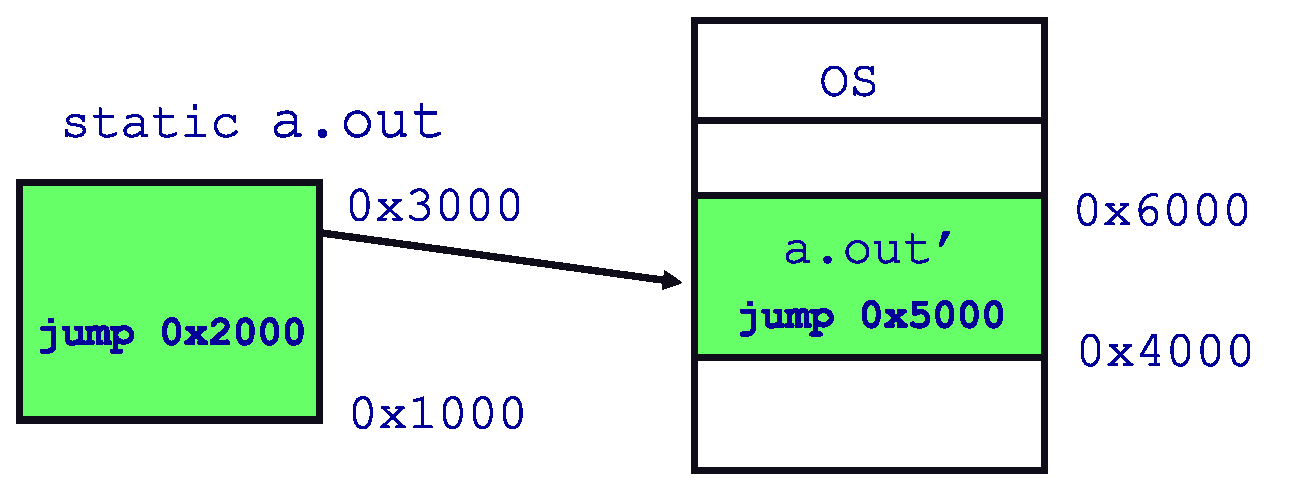
\includegraphics[height=1.3in]{figs/loadtime}}
\smallskip
\itms{
  \item Two special privileged registers:  \Red{base} and \Red{bound}
  \item On each load/store:
  \ittms{
    \item Physical address = virtual address + \Red{base}
    \item Check $0\le \mathrm{virtual\ address}<\mathrm{\Red{bound}}$, else
  trap to kernel
  }
  \item How to move process in memory?
  \ittms{
\onslide<2->{
    \item Change \Red{base} register
   }
  }
  \item What happens on context switch?
  \ittms{
\onslide<3->{
    \item OS must re-load \Red{base} and \Red{bound} register
}
  }
}
\end{slide}

\begin{slide}{Definitions}
\itms{
  \item Programs load/store to \Red{virtual} (or \Red{logical})
    \Red{addresses}
  \item Actual memory uses \Red{physical} (or \Red{real})
    \Red{addresses}
  \item VM Hardware is Memory Management Unit (\Red{MMU}) \\
  \ittms{
    \item[] 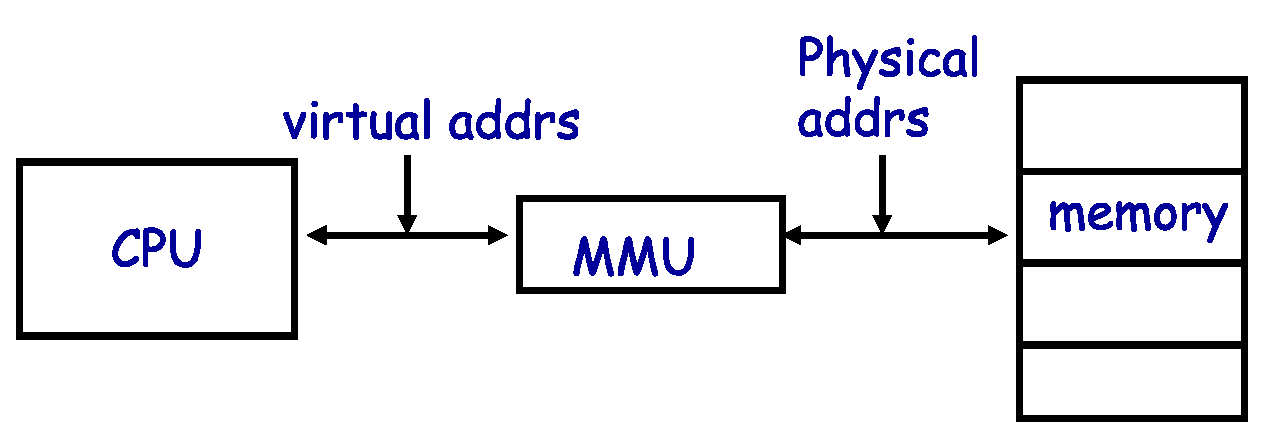
\includegraphics[width=96mm]{figs/mmu}
    \item Usually part of CPU
    \item Accessed w.\ privileged instructions (e.g., load bound reg)
    \item Translates from virtual to physical addresses
    \item Gives per-process view of memory called \Red{address space}
  }
}
\end{slide}

\begin{slide}{Address space}
\centerline{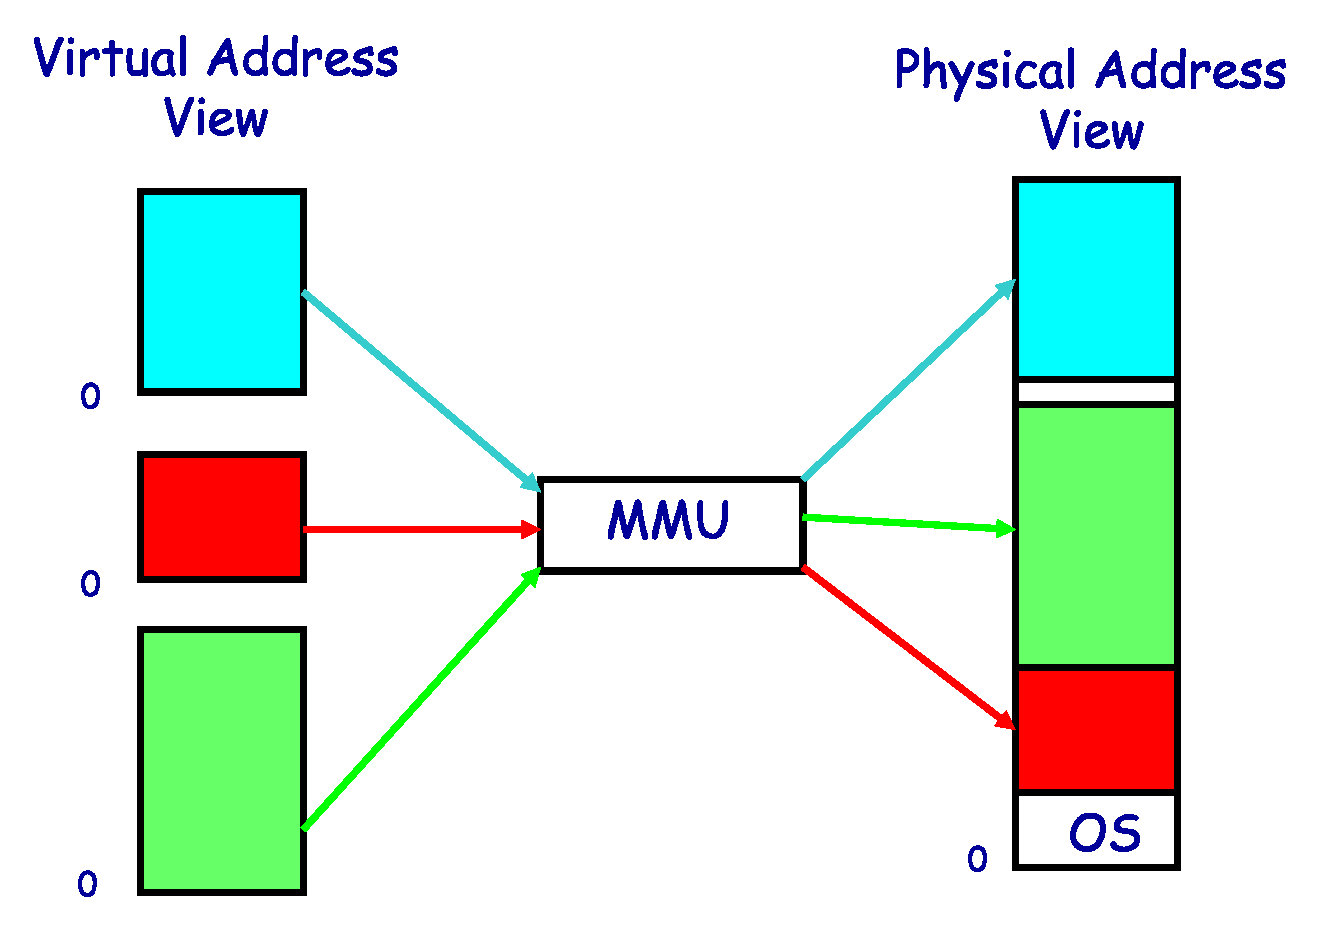
\includegraphics[width=4in]{figs/addressspace}}
\end{slide}

\begin{slide}{Base+bound trade-offs}
\itms{
\item Advantages
\ittms{
  \item Cheap in terms of hardware: only two registers
  \item Cheap in terms of cycles: do add and compare in parallel
  \item Examples: Cray-1 used this scheme
}
}
\begin{columns}[T,onlytextwidth]
\column{83mm}
\itms{
  \item Disadvantages
  \ittms{
    \item Growing a process is expensive or impossible
    \item No way to share code or data 
          (E.g., two copies of bochs)
  }
}
\column{25mm}
%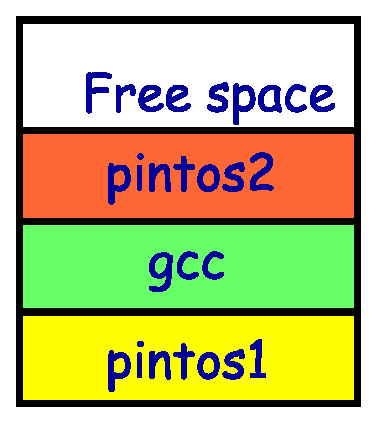
\includegraphics[width=25mm]{figs/bbtradeoff}
\end{columns}
\itms{
  \item One solution:  Multiple segments
  \ittms{
    \item E.g., separate code, stack, data segments
    \item Possibly multiple data segments
}}
\end{slide}

\section{Segmentation}

\begin{slide}{Segmentation}
\centerline{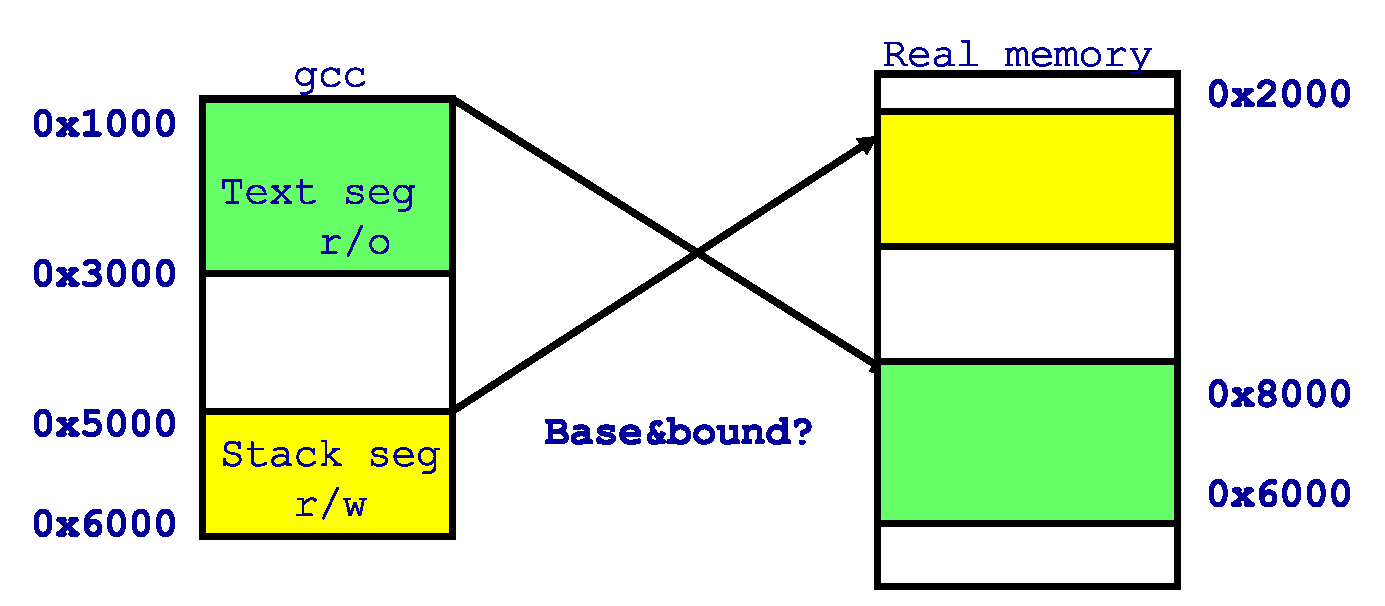
\includegraphics[height=2in]{figs/segmentation}}
\itms{
  \item Let processes have many base/bound regs
  \ittms{
    \item Address space built from many segments
    \item Can share/protect memory at segment granularity
  }
  \item Must specify segment as part of virtual address
}
\end{slide}

\begin{slide}{Segmentation mechanics}
\centerline{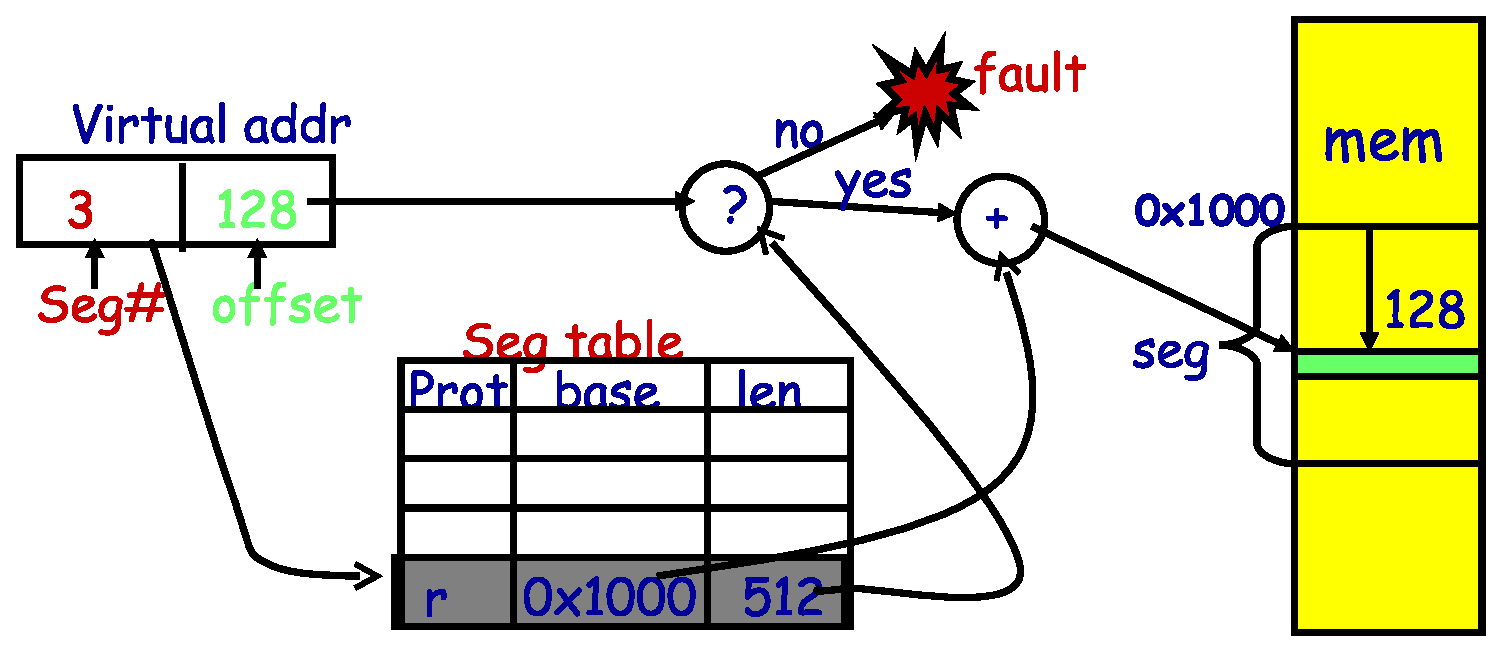
\includegraphics[height=1.8in]{figs/seg-mech}}
\itms{
\item Each process has a segment table
\item Each VA indicates a segment and offset:
\ittms{
  \item Top bits of addr select segment, low bits select offset
    (PDP-10)  
  \item Or segment selected by instruction or operand (means you need
    wider ``far'' pointers to specify segment)
}
}
\end{slide}

\begin{slide}{Segmentation example}
\centerline{\includegraphics[height=2.5in]{seg-example}}
\itms{
  \item 2-bit segment number (1st digit), 12 bit offset (last 3)
  \ittms{
    \item Where is 0x0240? 0x1108? 0x265c? 0x3002? 0x1600?
  }
}
\end{slide}

\begin{slide}{Segmentation trade-offs}
\hbox{
\begin{minipage}{3in}
\vspace*{-.5in}
\itms{
  \item Advantages
  \ittms{
    \item Multiple segments per process
    \item Allows sharing!  (how?)
    \item Don't need entire process in memory
  }
}
\end{minipage}
\begin{minipage}{1in}
%\vspace*{-.2in}
\centerline{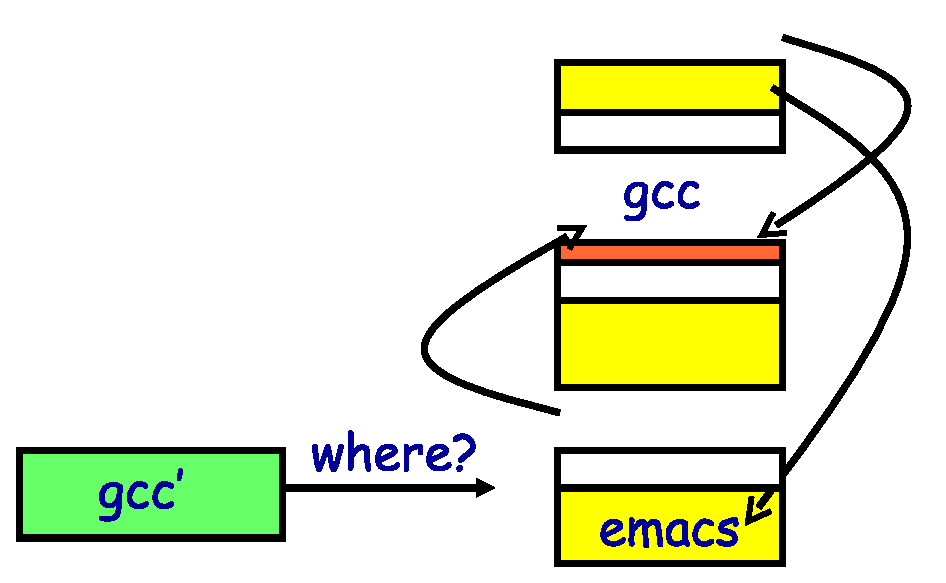
\includegraphics[height=1.5in]{figs/segtradeoff}\hspace*{.5in}}
\end{minipage}
}
\vspace*{-.3in}
\itms{
\item Disadvantages
\ittms{
\item Requires translation hardware, which could limit performance
\item Segments not completely transparent to program (e.g., default
  segment faster or uses shorter instruction)
\item $n$ byte segment needs $n$ \emph{contiguous} bytes of
physical memory
\item Makes \emph{fragmentation} a real problem.
}
}
\end{slide}

\begin{slide}{Fragmentation}
\vspace*{-.1in}
\itms{
\item \Red{Fragmentation} $\rightarrow$ Inability to use free memory
\item Over time:
\ittms{
  \item Variable-sized pieces = many small holes (external
  fragmentation)
  \item Fixed-sized pieces = no external holes, but force internal waste
   (internal fragmentation)
}
}
\centerline{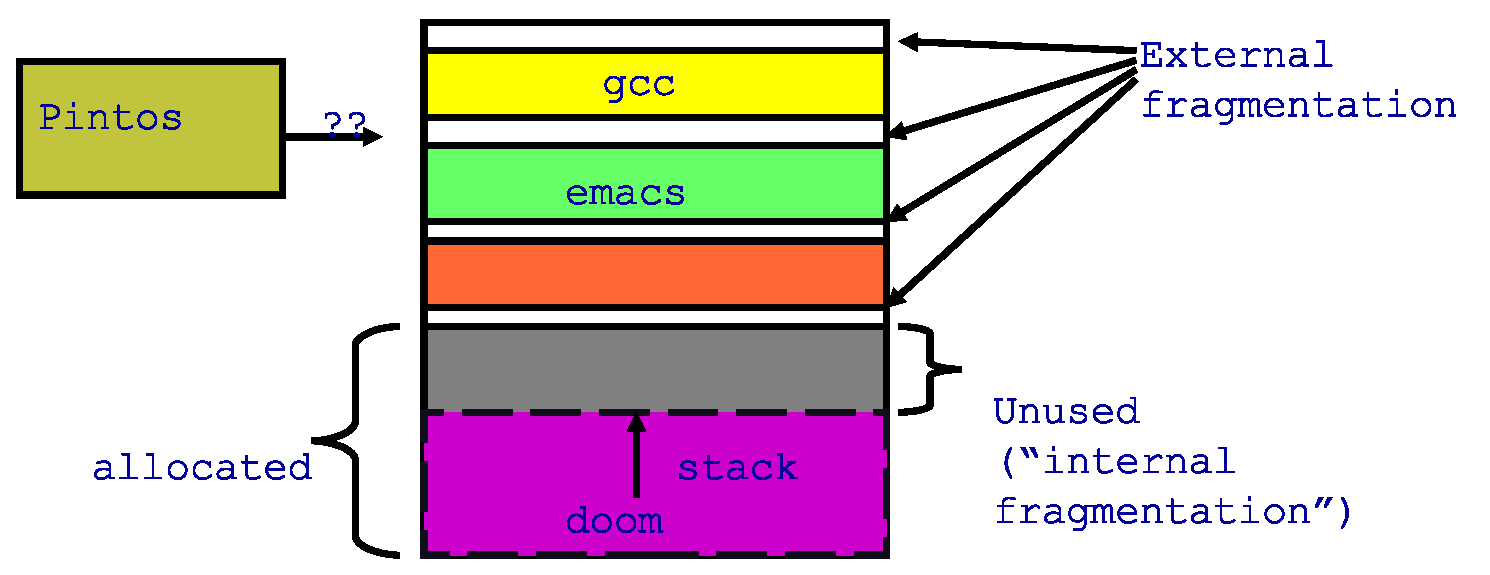
\includegraphics[width=4in]{figs/fragmentation}}
\end{slide}

% Bring me back later
%  \begin{slide}{Alternatives to hardware MMU}
%  \itms{
%  %  \item Segmentation
%  %  \ittms{
%  %    \item Part of each memory reference implicit in segment register\\
%  %	  $\mbox{segreg}\gets\langle\mathrm{offset,limit}\rangle$
%  %    \item By loading segment register code can be relocated
%  %    \item Can enforce protection by restricting segment register loads
%  %  }
%    \item Language-level protection (Java)
%    \ittms{
%      \item Single address space for different modules
%      \item Language enforces isolation
%      \item Singularity OS does this
%        \href{http://research.microsoft.com/pubs/52716/tr-2005-135.pdf}{[Hunt]}
%    }
%    \bigskip
%    \item Software fault isolation
%    \ittms{
%      \item Instrument compiler output
%      \item Checks before every store operation prevents modules from
%  	  trashing each other
%      \item Google \href{http://code.google.com/p/nativeclient/}{Native Client}
%            does this with only about 5\% slowdown
%  \href{http://research.google.com/pubs/archive/34913.pdf}{[Yee]}
%    }
%  }
%  \end{slide}

\section{Paging}

\begin{slide}{Paging}
\itms{
  \item Divide memory up into small \emph{pages}
  \item Map virtual pages to physical pages
  \ittms{
    \item Each process has separate mapping
  }
  \item Allow OS to gain control on certain operations
  \ittms{
    \item Read-only pages trap to OS on write
    \item Invalid pages trap to OS on read or write
    \item OS can change mapping and resume application
  }
  \item Other features sometimes found:
  \ittms{
    \item Hardware can set ``accessed'' and ``dirty'' bits
    \item Control page execute permission separately from read/write
    \item Control caching or memory consistency of page
  }
}
\end{slide}

\begin{slide}{Paging trade-offs}
\centerline{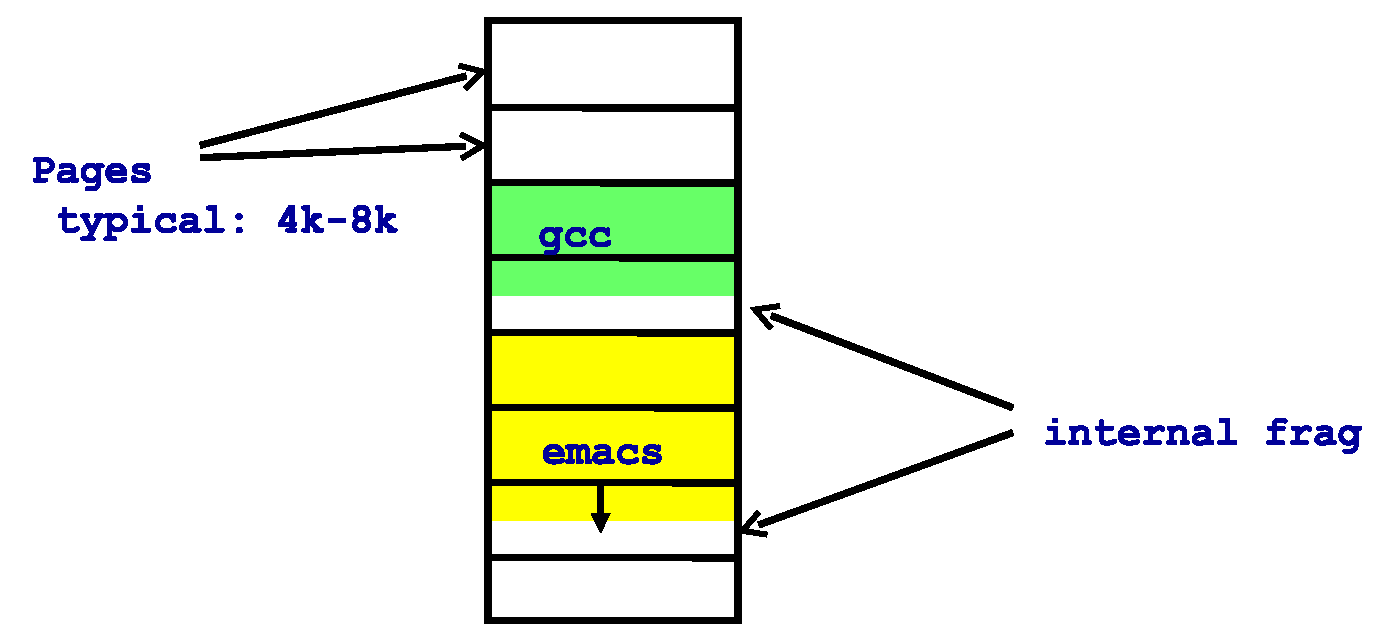
\includegraphics[width=4in]{figs/paging}}
\medskip
\itms{
  \item Eliminates external fragmentation
  \item Simplifies allocation, free, and backing storage (swap)
  \item Average internal fragmentation of .5 pages per ``segment''
}
\end{slide}

\begin{slide}{Simplified allocation}
\centerline{\documentclass[letterpaper,twocolumn,10pt]{article}

\usepackage[letterpaper, margin=1in, tmargin=1.5in]{geometry}
\usepackage{fancyhdr}
\usepackage{microtype}

\usepackage{booktabs}
\usepackage{xcolor}
\usepackage{listings}

\definecolor{lightgrey}{rgb}{0.95,0.95,0.95}

% VS2017 C++ color scheme
\definecolor{clr-background}{RGB}{255,255,255}
\definecolor{clr-text}{RGB}{0,0,0}
\definecolor{clr-string}{RGB}{163,21,21}
\definecolor{clr-namespace}{RGB}{0,0,0}
\definecolor{clr-preprocessor}{RGB}{128,128,128}
\definecolor{clr-keyword}{RGB}{0,0,255}
\definecolor{clr-type}{RGB}{43,145,175}
\definecolor{clr-variable}{RGB}{0,0,0}
\definecolor{clr-constant}{RGB}{111,0,138} % macro color
\definecolor{clr-comment}{RGB}{0,128,0}

\lstdefinestyle{CStyle}{
    language=C,
    % VS colors
    backgroundcolor=\color{clr-background},
    basicstyle=\small\ttfamily\color{clr-text},
    stringstyle=\color{clr-string},
    identifierstyle=\color{clr-variable},
    commentstyle=\color{clr-comment},
    directivestyle=\color{clr-preprocessor},
    keywordstyle=\color{clr-type},
    keywordstyle={[2]\color{clr-constant}},
    %frame=tb,
    captionpos=b,
    columns=fullflexible,
    %backgroundcolor=\color{lightgrey},
    showstringspaces=false,
    keepspaces=true,
    tabsize=8,
    numbers=left,
    numbersep=5pt,
    linewidth=0.7\textwidth
}

\lstset{style=CStyle}

\begin{document}

\pagestyle{fancy}
\fancyhead[L]{\bf CS350: Operating Systems}
\fancyhead[R]{\bf Paging}
\fancyfoot[C]{\thepage}

Consider a paging-based virtual memory system with 32-bit virtual and physical 
adresses, and a page size of $2^{12}$ bytes (4~KiB).  Suppose that a process P 
is running. P uses only 128~KiB of virtual memory.  The first 5 entries of P's 
page table are shown below.

\begin{table}
\centering
\begin{tabular}{l|l|c}
\toprule
Page \# & Frame \# & Valid \\
\midrule
0x0 & 0x00234 & 1\\
    0x1 & 0x00235 & 1\\
    0x2 & 0x0023f & 1\\
    0x3 & 0x00ace & 1\\
    0x4 & 0x00004 & 1\\
\bottomrule
\end{tabular}
\end{table}

\vspace{4em}

\noindent
\textbf{Question 1.} What is the total number of entries in P's page table?

\vspace{16em}

\noindent
\textbf{Question 2.} How many entries are valid?

\vspace{16em}
\break

\textbf{Question 3.} What physical addresses correspond to each of these 
virtual addresses?

\begin{itemize}
\item 0x00001a60
\item 0x00000fb5
\item 0x00004664
\end{itemize}

\vspace{16em}

\textbf{Question 4.} If the page size were 16~KiB instead of 4~KiB, how many 
entries would there be in P's page table?  How many bits of each virtual 
address would be used for the offset, and how many for the page number?

\end{document}

}
\itms{
  \item Allocate any physical page to any process
  \item Can store idle virtual pages on disk
}
\end{slide}

\begin{slide}{Paging data structures}
\vspace*{-2mm}
\itms{
  \item Pages are fixed size, e.g., 4K
  \ittms{
    \item Least significant 12 ($\log_2$ 4K) bits of address are
      \emph{page offset}
    \item Most significant bits are \emph{page number}
  }
  \item Each process has a \emph{page table}
  \ittms{
    \item Maps \emph{virtual page numbers} (VPNs) to \emph{physical
    page numbers} (PPNs)
    \item Also includes bits for protection, validity, etc.
  }
  \item On memory access:  Translate VPN to PPN, \\
        then add offset
}
\vspace*{-5mm}
\centerline{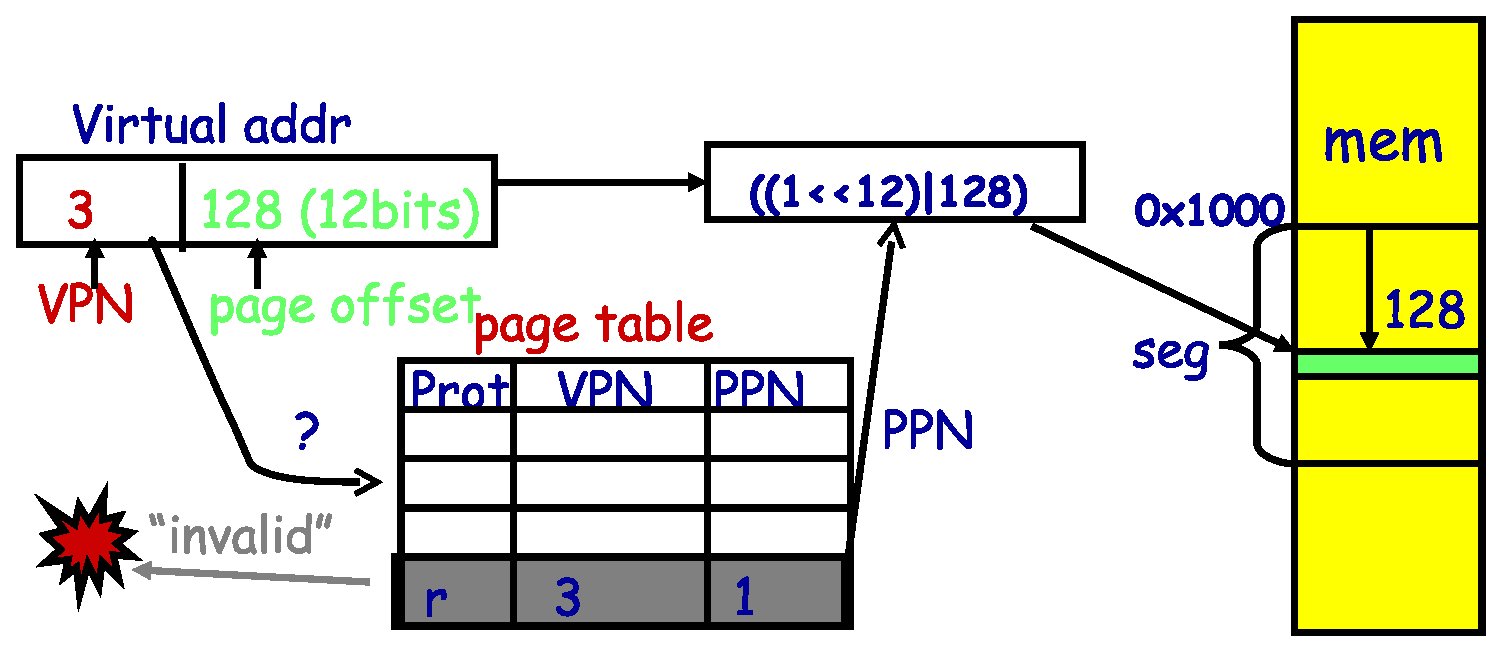
\includegraphics[width=3.5in]{figs/page-mech}}
\end{slide}

\begin{slide}{Example: Paging on PDP-11}
\itms{
  \item 64K virtual memory, 8K pages
  \ittms{
    \item Separate address space for instructions \& data
    \item I.e., can't read your own instructions with a load
  }
  \medskip
  \item Entire page table stored in registers
  \ittms{
    \item 8 Instruction page translation registers
    \item 8 Data page translations
  }
  \medskip
  \item Swap 16 machine registers on each context switch
}
\end{slide}

%% \begin{slide}{Example: VAX}
%% \itms{
%%   \item Virtual memory partitioned
%%   \ittms{
%%     \item First 2 Gigs for applications
%%     \item Last 2 Gigs for OS---mapped same in all address spaces
%%     \item One page table for system memory, one for each process
%%   }
%%   \item Each user page table is 8 Megabytes
%%   \ittms{
%%     \item 512-byte pages, 4 bytes/translation, \\
%% 	1~Gig for application (not counting stack)
%%   }
%%   \item User page tables stored in paged kernel memory
%%   \ittms{
%%     \item No need for 8 physical Megs/proc. only virtual
%%   }
%% }
%% \end{slide}

\begin{slide}{MMU Types}
  \itms{
    \item Memory Management Units (MMU) come in two flavors
    \item Hardware Managed
    \ittms{
      \item Hardware reloads TLB with pages from a page tables
      \item Typically hardware page tables are Radix Trees
      \item Requires complex hardware
      \item Examples: x86, ARM64, IBM POWER9+
    }
    \item Software Managed
    \ittms{
      \item Simplier hardware and asks software to reload pages
      \item Requires fast exception handling and optimized software
      \item Enables more flexiblity in the TLB (e.g. variable page sizes)
      \item Examples: MIPS, Sun SPARC, DEC Alpha, ARM and POWER
    }
  }
  \end{slide}
  
  \section{Intel x86: Hardware MMU}
  
  \begin{slide}{x86 Paging}
  \itms{
    \item Paging enabled by bits in a control register (\texttt{\%cr0})
    \ittms{
      \item Only privileged OS code can manipulate control registers
    }
    \item Normally 4KB pages
    \item \texttt{\%cr3}: points to 4KB page directory
    \item Page directory: 1024 PDEs (page directory entries)
    \ittms{
      \item Each contains physical address of a page table
    }
    \item Page table: 1024 PTEs (page table entries)
    \ittms{
      \item Each contains physical address of virtual 4K page
      \item Page table covers 4 MB of Virtual mem
    }
    \item See intel manual for detailed explanation
    \ittms{
      \item Volume 2 of
        \href{http://developer.amd.com/Resources/documentation/guides/Pages/default.aspx\#manuals}{AMD64 Architecture docs}
      \item Volume 3A of
        \href{http://www.intel.com/content/www/us/en/processors/architectures-software-developer-manuals.html}{Intel Pentium Manual}
    }
  }
  \end{slide}
  
  \begin{slide}{x86 page translation}
  \begin{figure}
  \centering
  \input{x86.tex}
  \end{figure}
  \end{slide}
  
  \begin{slide}{x86 page directory entry}
  \bigskip
  \begin{figure}
  \centering
  \input{pde.tex}
  \end{figure}
  \end{slide}
  
  \begin{slide}{x86 page table entry}
  \bigskip
  \begin{figure}
  \centering
  \input{pte.tex}
  \end{figure}
  \end{slide}
  
  \begin{slide}{x86 hardware segmentation}
  \itms{
    \item x86 architecture \emph{also} supports segmentation
    \ittms{
      \item Segment register base + pointer val = \emph{linear address}
      \item Page translation happens on linear addresses
    }
    \item Two levels of protection and translation check
    \ittms{
      \item Segmentation model has four privilege levels (CPL 0--3)
      \item Paging only two, so 0--2 = kernel, 3 = user
    }
    \item Why do you want \emph{both} paging and segmentation?
  \pause
    \item Short answer:  You don't -- just adds overhead
    \ittms{
      \item Most OSes use ``flat mode'' -- set base = 0, bounds =
        0xffffffff \\
        in all segment registers, then forget about it
      \item x86-64 architecture removes much segmentation support
    }
    \item Long answer:  Has some fringe/incidental uses
    \ittms{
      \item VMware runs guest OS in CPL 1 to trap stack faults
      \item OpenBSD used CS limit for W$\wedge$X when no PTE NX bit
    }
  }
  \end{slide}
  
  \begin{slide}{Making paging fast}
  \itms{
    \item x86 PTs require 3 memory references per load/store
    \ittms{
      \item Look up page table address in page directory
      \item Look up PPN in page table
      \item Actually access physical page corresponding to virtual
    address
    }
    \item For speed, CPU caches recently used translations
    \ittms{
      \item Called a \emph{translation lookaside buffer} or \Red{TLB}
      \item Typical: 64-2K entries, 4-way to fully associative, 95\% hit rate
      \item Each TLB entry maps a VPN $\to$ PPN + protection information
    }
    \item On each memory reference
    \ittms{
      \item Check TLB, if entry present get physical address fast
      \item If not, walk page tables, insert in TLB for next time \\
        (Must evict some entry) 
    }
  }
  \end{slide}
  
  \begin{slide}{TLB details}
  \itms{
  \item TLB operates at CPU pipeline speed $\rightarrow$ small, fast
  \item Complication: what to do when switch address space?
  \ittms{
    \item Flush TLB on context switch (e.g., old x86)
    \item Tag each entry with associated process's ID (e.g., MIPS)
  }
  \item In general, OS must manually keep TLB valid
  \item E.g., x86 \emph{invlpg} instruction
    \ittms{
     \item Invalidates a page translation in TLB
     \item Must execute after changing a possibly used page table entry
     \item Otherwise, hardware will miss page table change
    }
  \item More Complex on a multiprocessor (TLB shootdown)
  %\item TLB reload can be done to hardware or software
  %\ittms{
  %  \item Hardware - x86 walks page tables on miss.
  %  \item Software - MIPS - trap to OS to reload.
  %     OS get to decide "page table" format
  }
  \end{slide}
  
%  \begin{slide}{x86 Paging Extensions}
%  \itms{
%    \item PSE: Page size extensions
%    \ittms{
%      \item Setting bit 7 in PDE makes a 4MB translation (no PT)
%    }
%    \item PAE Page address extensions
%    \ittms{
%      \item Newer 64-bit PTE format allows 36 bits of physical address
%      \item Page tables, directories have only 512 entries
%      \item Use 4-entry Page-Directory-Pointer Table to regain 2 lost bits
%      \item PDE bit 7 allows 2MB translation
%    }
%    \item Long mode PAE
%    \ittms{
%       \item In Long mode, pointers are 64-bits
%       \item Extends PAE to map 48 bits of virtual address (next slide)
%       \item Why are aren't all 64 bits of VA usable?
%    }
%  }
%  \end{slide}
  
%  \begin{slide}{x86 long mode paging}
%  \hspace*{-4mm}\input{long.tex}
%  % \itms{
%  %   \item Why are aren't upper 16 bits of VA used?
%  % % Table walking is slow, would hurt performance
%  % }
%  \end{slide}
  
  \begin{slide}{Where does the OS live?}
  \itms{
    \item In its own address space?
    \ittms{
      \item Can't do this on most hardware
             (e.g., syscall instruction won't switch address spaces)
      \item Also would make it harder to parse syscall arguments passed
    as pointers
    }
    \item So in the same address space as process
    \ittms{
      \item Use protection bits to prohibit user code from writing
    kernel
    }
    \item Typically
      all kernel text, most data at same VA in every address space
    \ittms{
      \item On x86, must manually set up page tables for this
      \item Usually just map kernel in contiguous virtual memory when
    boot loader puts kernel into contiguous physical memory
      \item Some hardware puts physical memory (kernel-only) somewhere in virtual
    address space
    }
  }
  \end{slide}
  
  \section{MIPS: Software Managed MMU}
  
  \begin{slide}{Very different MMU: MIPS}
  \itms{
    \item Hardware has 64-entry TLB
    \ittms{
      \item References to addresses not in TLB trap to kernel
    }
    \item Each TLB entry has the following fields:\\
      {\mdseries\scriptsize Virtual page, Pid, Page frame, NC, D, V, Global}
    \item Kernel itself unpaged
    \ittms{
      \item All of physical memory contiguously mapped in high VM
      \item Kernel uses these pseudo-physical addresses
    }
    \item User TLB fault hander very efficient
    \ittms{
      \item Two hardware registers reserved for it
      \item utlb miss handler can itself fault---allow paged page tables
    }
    \item OS is free to choose page table format!
  }
  \end{slide}
  
  \newcommand{\descbox}[2]{\parbox[c][3.8\baselineskip]{0.95\width}{%
    \raggedright #1\vfill #2}}
  \newcommand{\memsection}[4]{%
    % define the height of the memsection
    \bytefieldsetup{bitheight=#3\baselineskip}%
    \bitbox[]{10}{%
      \texttt{#1}%print end address
      \\
      % do some spacing
      \vspace{#3\baselineskip}
      \vspace{-2\baselineskip}
      \vspace{-#3pt}
      \texttt{#2}%print start address
    }%
    \bitbox{16}{#4}%    print box with caption
  }
  
  \begin{slide}{MIPS Memory Layout}
  \begin{bytefield}{16}
    \begin{rightwordgroup}{Kernel Memory}
    \memsection{FFFF FFFF}{C000 0000}{4}{kseg2: Paged Kernel}\\
    \memsection{BFFF FFFF}{A000 0000}{2}{kseg1: Phys. Uncached}\\
    \memsection{9FFF FFFF}{8000 0000}{2}{kseg0: Phys. Cached}
    \end{rightwordgroup}\\
    \begin{rightwordgroup}{User Memory}
    \memsection{7FFF FFFF}{0000 0000}{8}{useg: Paged User}
    \end{rightwordgroup}
  \end{bytefield}
  \end{slide}
  
  \begin{slide}{MIPS Translation Lookaside Buffer}
  \itms{
    \item TLB Entries: 64 - 64-bit entries containing:
    \ittms{
    \item PID: Process ID (tagged TLB)
    \item N: No Cache - disables caching for memory mapped I/O
    \item D: Writeable - makes the page writeable
    \item V: Valid
    \item G: Global - ignores the PID during lookups
    }
  }
  \vspace{1em}
  \begin{bytefield}[endianness=big,bitwidth=0.9em]{64}
    \bitheader{32-63} \\
    \bitbox{20}{Frame Number (VPN)} &
    \bitbox{6}{PID} &
    \bitbox{6}{} \\
  \end{bytefield}
  \begin{bytefield}[endianness=big,bitwidth=0.9em]{32}
    \bitheader{0-31} \\
    \bitbox{20}{Physical Page Number (PPN)} &
    \bitbox{1}{N}
    \bitbox{1}{D}
    \bitbox{1}{V}
    \bitbox{1}{G}
    \bitbox{8}{} \\
  \end{bytefield}
  \vspace{-1em}
  \itms{
    \item Page Sizes: Multiples of 4 from 4~kiB--16~MiB
    \ittms{
      \item 4~kiB, 16~kiB, 64~kiB, 256~kiB, 1~MiB, 4~MiB, 16~MiB
    }
  }
  \end{slide}
  
  \begin{slide}{TLB PID and Global Bit}
  \itms{
    \item Process ID (PID) allows multiple processes to coexist
    \ittms{
      \item We don't need to flush the TLB on context switch
      \item By setting the process ID 
      \item Only flush TLB entries when reusing a PID
      \item Current PID is stored in {\tt c0\_entryhi}
    }
    \medskip
    \item Global bit
    \ittms{
      \item Used for pages shared across all address spaces in kseg2 or useg
      \item Ensures the TLB ignores the PID field
      \item Typically in most hardware a TLB flush doesn't flush global pages
    }
  }
  \end{slide}
  
  \begin{slide}{TLB Instructions}
  \itms{
    \item MIPS co-processor 0 (COP0) provides the TLB functionality
    \medskip
    \item Four instructions:
    \ittms{
      \item {\tt tlbwr}: TLB write a random slot
      \item {\tt tlbwi}: TLB write a specific slot
      \item {\tt tlbr}: TLB read a specific slot
      \item {\tt tlbp}: Probe the slot containing an address
    }
    \medskip
    \item For each of these instructions you must load the following registers
    \ittms{
      \item {\tt c0\_entryhi}: high bits of TLB entry
      \item {\tt c0\_entrylo}: low bits of TLB entry
      \item {\tt c0\_index}: TLB Index
    }
  }
  \end{slide}
  
  \begin{slide}{Hardware Lookup Exceptions}
  \itms{
    \item TLB Exceptions:
    \ittms{
      \item UTLB Miss: Generated when the accessing useg without matching TLB 
        entry
      \item TLB Miss: Generated when the accessing kseg2 without matching entry
      \item TLB Mod: Generated when writing to read-only page
    }
    \medskip
    \item UTLB handler is seperate from general exception handler
    \ittms{
      \item UTLBs are very frequent and require a hand optimized path
      \item 64 entry TLB with 4~kiB pages covers 256~kiB of memory
      \item Modern machines have workloads with far more memory
      \item Require more entries (expensive hardware) or larger pages
    }
  }
  \end{slide}
  
  \begin{slide}{Hardware Lookup Algorithm}
  \itms{
  \item If most significant bit (MSB) is 1 and in user mode $\rightarrow$ address 
    error exception.
    \item If no VPN match $\rightarrow$ TLB miss exception if MSB is 1, otherwise 
      UTLB miss.
    \item If PID mismatches and global bit not set $\rightarrow$ generate a TLB 
      miss or UTLB miss.
    \item If valid bit not set $\rightarrow$ TLB miss.
    \item Write to read-only page $\rightarrow$ TLB mod exception.
    \item If N bit is set directly access device memory (disable cache)
  }
  \end{slide}
  
  \begin{slide}{OS/161 Assembly Wrappers}
  \itms{
    \item {\tt tlb\_random}: Write random TLB entry
    \item {\tt tlb\_write}: Write specific TLB entry
    \item {\tt tlb\_read}: Read specific TLB entry
    \item {\tt tlb\_probe}: Lookup TLB entry
    \item Currently the OS implements segments using paging hardware
    \item In a later assignment you will implement a Radix tree (like x86)
  }
  \end{slide}
  
  \begin{slide}{OS/161 Memory Layout}
  \itms{
    \item Example Memory Layout: user/testbin/sort
  }
  \begin{bytefield}{15}
    \memsection{7FFF FFFF}{xxxx xxxx}{2}{Stack}\\
    \memsection{}{}{6}{}\\
    \memsection{1012 00B0}{1000 0000}{2}{Data}\\
    \memsection{}{}{2}{}\\
    \memsection{0040 1A0C}{0040 0000}{2}{Text + R/O Data}\\
    \memsection{}{}{1}{}\\
  \end{bytefield}
  \end{slide}
  
  %\begin{slide}{DEC Alpha MMU}
  %\itms{
  %  \item Software managed TLB (like MIPS)
  %  \ittms{
  %    \item 8KB, 64KB, 512KB, 4MB pages all available
  %    \item TLB supports 128 instruction/128 data entries of any size
  %  }
  %  \item But TLB miss handler not part of OS
  %  \ittms{
  %    \item Processor ships with special ``PAL code'' in ROM
  %    \item Processor-specific, but provides uniform interface to OS
  %    \item Basically firmware that runs from main memory like OS
  %  }
  %  \item Various events vector directly to PAL code
  %  \ittms{
  %    \item \texttt{call\_pal} instruction, TLB miss/fault, FP disabled
  %  }
  %  \item PAL code runs in special privileged processor mode
  %  \ittms{
  %    \item Interrupts always disabled
  %    \item Have access to special instructions and registers
  %  }
  %}
  %\end{slide}
  %
  %\begin{slide}{PAL code interface details}
  %\itms{
  %  \item Examples of Digital Unix PALcode entry functions
  %  \ittms{
  %    \item \texttt{callsys}/\texttt{retsys} - make, return from system call
  %    \item \texttt{swpctx} - change address spaces
  %    \item \texttt{wrvptptr} - write virtual page table pointer
  %    \item \texttt{tbi} - TBL invalidate
  %  }
  %  \item Some fields in PALcode page table entries
  %  \ittms{
  %    \item GH - 2-bit granularity hint $\to 2^N$ pages have same translation
  %    \item ASM - address space match $\to$ mapping applies in all processes
  %  }
  %}
  %\end{slide}
  %
  %\begin{slide}{Example:  Paging to disk}
  %\itms{
  %  \item \texttt{gcc} needs a new page of memory
  %  \item OS re-claims an idle page from \texttt{emacs}
  %  \item If page is \emph{clean} (i.e., also stored on disk):
  %  \ittms{
  %    \item E.g., page of text from emacs binary on disk
  %    \item Can always re-read same page from binary
  %    \item So okay to discard contents now \& give page to \texttt{gcc}
  %  }
  %  \item If page is \emph{dirty} (meaning memory is only copy)
  %  \ittms{
  %    \item Must write page to disk first before giving to \texttt{gcc}
  %  }
  %  \item Either way:
  %  \ittms{
  %    \item Mark page invalid in \texttt{emacs}
  %    \item \texttt{emacs} will fault on next access to virtual page
  %    \item On fault, OS reads page data back from disk into new page, maps
  %  new page into \texttt{emacs}, resumes executing
  %  }
  %}
  %\end{slide}
  
  \begin{slide}{Paging in day-to-day use}
  \itms{
    \item Paging Examples
    \ittms{
    \item Demand paging
    \item Growing the stack
    \item BSS page allocation
    \item Shared text
    \item Shared libraries
    \item Shared memory
    \item Copy-on-write (\texttt{fork}, \texttt{mmap}, etc.)
    }
    \item Next time: detailed discussion on operating system side
  }
  \end{slide}

\end{document}
